\documentclass[10pt]{exam}
\usepackage[phy]{template-for-exam}
\usepackage{hyperref,graphicx,tikz}
\usetikzlibrary{arrows.meta}

\title{Energy Skate Park Simulation}
\author{Rohrbach}
\date{\today}

\begin{document}
\maketitle


\noindent
Go to \texttt{\href{https://phet.colorado.edu/en/simulations/energy-skate-park-basics}{https://phet.colorado.edu/en/simulations/energy-skate-park-basics}} and click the Play button.

\begin{questions}

\question
	Select the picture that says ``Intro.''  Turn on all the checkboxes on the upper right part of the screen. Place your skater at the beginning of the track and allow her to move on the track a few times.  What do you notice about the height of the skater at the beginning and end of motion?  Why do you think this is?
  
  \begin{flushright}
    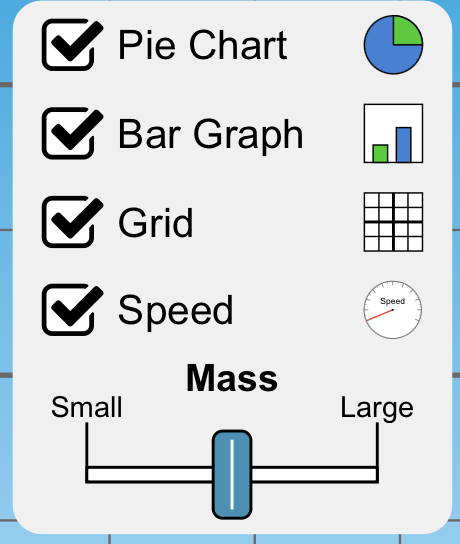
\includegraphics[width=2cm]{PhET_checkboxes.png}
  \end{flushright}

\question
	What pattern do you notice for the kinetic and potential energies of the skater (the blue and green lines in the bar graph)?
  \vs

\question
	What is your skater doing when she has the most kinetic energy?  Explain why this makes sense given the formula $KE=\frac{1}{2}mv^2$.
  \vs 

\question
	Where does your skater have the most potential energy?  Explain why this makes sense given the formula $PE=mgh$.
  \vs 

\question
	Explain how your skater obeys the Law of Conservation of Energy.
  \vs 

\question
	So, conservation of energy means that the total energy does not change.  But when the skater was sitting on the ground, she had no energy.  So where did the energy come from?  Think about the equation $KE_i+PE_i+W=KE_f+PE_f$.
  \vs 

\pagebreak

\question
  Increase or decrease the mass of your skater.  What changes about her total energy?  Why do you think this is?
  \vs

\question
	Change the track to the ``W''-shaped track.  Put your skater on the track and let her go.  Did you notice any changes to her pattern of kinetic and potential energies?   Why do you think this is?
  
  \begin{flushright}
    \begin{tikzpicture}
      \node at (0,0) 
        {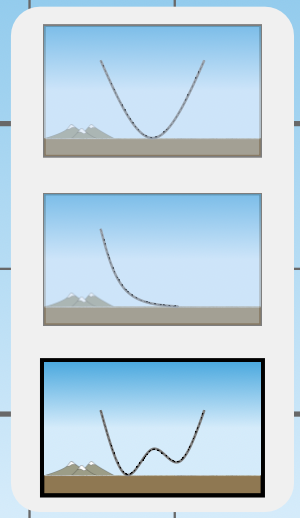
\includegraphics[width=2cm]{PhET_w.png}};
      \draw[ultra thick, rounded corners] 
        (-.8,-1.7) rectangle (.85,-.6);
      \draw[->,ultra thick,blue] (-1,-1.6) -- ++(0.4,0.4);
    \end{tikzpicture}
    
  \end{flushright}

\question
	Click on the ``friction'' picture at the bottom of the app.  Turn the bar graph and pie chart back on.  Start your skater in motion again.

  \begin{parts}

    \part
      What do you notice about the motion of your skater after turning on friction?
      
      \begin{flushright}
        \begin{tikzpicture}[scale=1.5]
          \node at (0,0) 
            {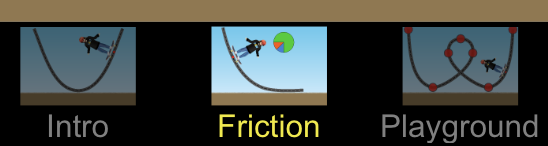
\includegraphics[height=1.5cm]{PhET_friction.png}};
          \draw[ultra thick, blue, rounded corners] 
            (-.7,-.6) rectangle (.7,.6);
        \end{tikzpicture}
      \end{flushright}

      \vspace{2em}

    \part
      If energy is conserved, then where does the total energy go since she eventually stops at the lowest point?
      \vs

    \part
      The simulation refers to \emph{thermal energy}, but we have not talked about that in class.  Take a look at the equation $KE_i+PE_i+W=KE_f+PE_f$ and think about which term corresponds to this \emph{thermal energy}.
      \vs
    
  \end{parts}


\question
	When you are finished with everything else, click on ``Playground'' mode at the bottom of the app.  Create a track that has a loop in it.  Play with the settings to investigate how energy is conserved in this case.  \emph{You do not need to write anything down for this question.}


\end{questions}


\end{document}